\chapter{Analysis and Theoretical Foundation}
\label{ch:analysis}
\pagestyle{fancy}

{\color{blue}Together with the next two chapters takes about 70\% of the whole paper.\\}

The purpose of this chapter is to explain the operating principles of the implemented
application.
Here you write about your solution from a theory standpoint – i.e. you explain it and demonstrate its theoretical properties/value, e.g.:
\begin{itemize}
	\item used or proposed algorithms,
    \item used protocols,
    \item  abstract models,
    \item  logic explanations/arguments concerning the chosen solution,
    \item  logic and functional structure of the application, etc.
\end{itemize}


~\\\parbox[c]{\textwidth}{\color{red}\bfseries

YOU SHOULD NOT write about the implementation.
YOU SHOULD NOT describe technologies and other things which do not pertain to
your project (no fillers, please!).
}


\section{A section title}\label{sec:context}

\subsection{A Subsection title}

Every table in the thesis should be numbered as Table \textit{x.y}, where \textit{x} is the chapter number where the table is included, and \textit{y} is the number of the table within that chapter. There should be one empty line after the paragraph preceding the table, and one empty line after the table. Example: in this row we have inserted a reference to Table~\ref{tab:nonlin}.

\begin{table}[ht]
    \caption{Results} % table caption
    \label{tab:nonlin} % \label{table:nonlin} introduces the label used to refer the table in the textt; reference is achieved via \ref{table:nonlin}
    \centering                          % centered table
    \begin{tabular}{|c|c|c|c|}          % 4 centerered columns
        \hline
        Case & Method\#1 & Method\#2 & Method\#3 \\ [0.5ex]   % heading
        \hline                              % single horizontal line
        1 & 50 & 837 & 970 \\               % table body
        2 & 47 & 877 & 230 \\
        3 & 31 & 25 & 415 \\[1ex]           % [1ex] adds vertical space
        \hline
    \end{tabular}

\end{table}

Every figure used in the thesis should be referred  (e.g. Figure x.y shows the components of the system...) and numbered.

Numbering is like this: Figure \textit{x.y} where \textit{x} is the chapter number and \textit{y} is the number of the figure within that chapter. E.g. , in this row we have inserted a reference to Figure~\ref{fig:imag}.

\begin{figure}[ht]
    \centering
    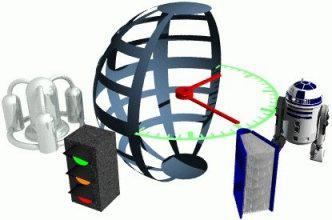
\includegraphics[]{figs/test.jpg}
    \caption{Figure name}
    \label{fig:imag}
\end{figure}

